\documentclass[../main.tex]{subfiles}
\begin{document}

\subsection{Structure of Euclidean Reflection Groups}

This section follows \cite{AbramenkoBrown2008}.

Let $W$ be an affine reflection group, naturally acting on the Euclidean space $V$, with fixed set of affine hyperplanes $\mathcal H$. We fix an arbitrary chamber $C$ as our fundamental chamber, $S$ be the set of reflection with respect to its walls. For an n-dimensional Euclidean space $V$, we have the isomorphism $\text{AO}(V) \cong V \rtimes \text{O}(V)$. Every element $\text{AO}(V)$ represents the composition of an orthogonal linear map with a transition $\tau_v$ sending $x$ to $x+v$. Note $W$ can be taken as a subgroup of $\text{AO}(V)$.

From Section \ref{Classification}, we recall some facts of affine reflection groups:\begin{enumerate}
    \item $W$ is generated by $S$.
    \item $W$ is simply transitive on chambers.
    \item $H\in \cH$ if and only if $s_H \in W$
    \item $\langle e_{s_i},e_{s_j}\rangle=-\cos(\frac{\pi}{m_{i,j}})$, where $e_{s_i},e_{s_j}$ are two unit vectors normal to some walls of $C$, pointing into $C$ from the walls. 
\end{enumerate}

\begin{theorem}\label{thm:finpara}
    \begin{enumerate}
        \item The hyperplanes $H\in \cH$ fall into finitely many classes under parallelism;
        \item Let $\overline W$ be the image of $W$ under the projection $\eta: \text{AO}(V) \twoheadrightarrow \text{O} (V)$, then $\overline W$ is finite.
    \end{enumerate}
\end{theorem}

\begin{proof}
    (1) Let $\Phi := \{\pm e_H:H\in \cH\}$, where $e_H$ is the unit vector normal to $H$. We will show $\angle(e_1,e_2)$ can take finitely many values. Let $H_1,H_2 \in \mathcal H$ normal to $e_1,e_2$. If they are parallel, then $\angle(e_1,e_2)=\pi$. So we may assume they intersect and take $x\in H_1\cap H_2$. Since $W$ is transitive on chambers, and by the fact that chambers $D,D'$ is separated by wall $H'$ if and only if $wD,wD'$ is separated by $wH'$, we can choose $w \in W$ with $wx\in \overline C$. Then $\overline C$ intersects with $wH_1$ and $wH_2$, with vectors $\bar we_1,\bar we_2$ normal to them, where $\bar w=\eta(w)$. $\angle(e_1,e_2)=\angle(\bar we_1,\bar we_2)$ since $\bar w$ is an isometry.   From the inner product formula we can deduce the angle between two distinct vectors cannot be smaller than $\pi/2$, so $C$ has finitely many walls. Then there are only finitely many possibilities for angles between two vectors in $\Phi$, hence it is finite as we are in a finite-dimensional space.

    (2) Note $\Phi$ we defined is stable under action of $\overline W$ and reflection with respect to the hyperplanes they are perpendicular to generates $\overline W$. We show the natural homomorphism $\sigma:\overline W \rightarrow S(\Phi)$ is injective. Suppose $w\in \text{ker}(\sigma)$, $w$ fixes all vectors of $\Phi$. But then $V_0=\text{Span}(\Phi)$ is also fixed by $w$. Write the vector space $V$ as $V_0\oplus V_1$ for $V_1$ some subspace of $V$. Then since every reflection $s_e$ fixes every point of $V_1$ and $W$ is generated by reflection of walls of $C$, so does $w$. We then conclude $w$ is identity hence $\overline W$ is finite.
\end{proof}

\begin{definition}
    We say $W$ is essential if intersection of hyperplanes $H$ $s_H \in \overline W$ is a singleton.
\end{definition}

\begin{definition}
    A Coxeter group is irreducible if its Coxeter diagram is connected.
\end{definition}

For a general affine reflection group, we can reduce it to essential, irreducible cases. If it is irreducible, then there are sets of hyperplanes $\cH_i$, each hyperplane in $\cH_i$ is orthogonal to the ones in other $\cH_j$'s. We can decompose the space into direct sum $V_1 \oplus \dots \oplus V_n$, where each $V_i$ corresponds to $\cH_i$, and the corresponding reflection group $W_i$ is irreducible in $V_i$. If $W_i$ is not essential, we can quotient the intersection of all hyperplanes out to get an essential one.

\begin{theorem}\label{thm:indep}
    Assume $W$ is essential and irreducible in $n$-dimensional vector space $V$, then one of the following is true:\begin{enumerate}
        \item $W$ is finite, $C$ has $n$ walls;
        \item $W$ is infinite, $C$ has $n+1$ walls, and vectors perpendicular to any $n$ walls form a basis. $\overline C$ is compact.
    \end{enumerate}
\end{theorem}

\begin{proof}
    We first count the number of walls. Suppose the walls of $C$ are $H_1,\dots,H_k$, with corresponding normal vectors $e_1,\dots,e_k$ pointing to $C$. Since $W$ is essential, $e_1,\dots,e_k$ is a spanning set hence $k\geq n$.

    Suppose $k=n$. Then the intersection of all $H_i$'s is a singleton. By shifting the planes we may assume $x=0$. Hence all $H_i$'s are linear and $W$ is a finite reflection group.

    Suppose $k>n$, then the list of vectors must be linearly dependent. Choose an index set $I$ such that \[
    \sum_{i\in I} \lambda_i e_i=0
    \]
    such that $\lambda_i \neq 0$ for all $i\in I$. We show $I=\{1,\dots,k\}$. Suppose not, then let $J=\{1,\dots,k\}\backslash I$. 

    Starting from $\sum_{i\in I} \lambda_i e_i=0$, move the negative coefficients terms to the right \[
    \sum_{i\in K} \lambda_i e_i=\sum_{i\in L} -\lambda_i e_i
    \] where $K,L$ is a partition of $I$.
    Then consider the inner product of left with right, since $\langle e_i,e_j \rangle$, it is non-positive. But it is also an inner product of two same vectors, then the summation is the $0$ vector.

    Choose $j\in J$ and take inner product \[
    \sum_{i\in K} \lambda_i \langle e_i,e_j\rangle =0
    \]
    For $i\in K$ $\lambda_i$ are positive and $\langle e_i,e_j\rangle$ are non-positive, we must have the case that $\langle e_i,e_j\rangle=0$, which implies $s_{e_i}s_{e_j}$ has order $2$. Then same thing holds for index set $L$. We then conclude the graph of $I$ and $J$ in Coxeter diagram are disconnected, contradicting irreducibility.

    $C$ now has $n+1$ walls, so $C$ is a bounded set. In particular $\overline C$ is compact. Since $W$ is simply transitive, $\bigcup_{w\in W} w\overline C$ is compact if $W$ is finite, but this union covers $V$ so $W$ is infinite.
\end{proof}

\begin{definition}
    A Euclidean reflection group is an essential, infinite, irreducible, affine reflection group.
\end{definition}

For the rest of this section, let $W$ be a Euclidean reflection group. Let $T$ be the kernel of the projection above restricted on $W$, then we have a short exact sequence \[
1\rightarrow T\rightarrow W \rightarrow\overline W \rightarrow 1
\]

\begin{proposition}\label{prop:special}
    There exists point $x\in V$ such that its group of stabilizers $W_x$ is isomorphic to $\overline W$. In particular, $W\cong T\rtimes W_x$.
\end{proposition}

\begin{proof}
    By Theorem \ref{thm:finpara}, let $\overline {\cH}$ be the set of linear hyperplanes parallel to some affine planes of $\cH$. $\overline W$ is generated by reflection about these hyperplanes. In fact $W$ is generated by $\{s_{\overline{H_1}},\dots,s_{\overline{H_n}}\}$, with $\overline{H_1},\dots,\overline{H_n} \in \overline {\cH}$. Choose affine hyperplanes $H_1,\dots,H_n$ from $\cH$, $H_i$ parallel to $\overline{H_i}$, and take their intersection, which is a single point $x$ by Theorem \ref{thm:indep}. Linear parts of $s_{H_1},\dots s_{H_n}$ generates $\overline W$ and since translations have no fixed points, $W_x$ bijects to $\overline W$.
\end{proof}

By Proposition \ref{prop:special}, with possibly shifting we can assume $0$ is a special point and hence $W\cong T\rtimes W_0\cong T \rtimes \overline W$. We can then identify $T$ by \[
L := \{v \in V : \tau_v \in W\}
\]
as a additive group. 

We then have $W\cong L\rtimes \overline W\leq V \rtimes \text{O}(V)\cong \text{AO}(V)$
We next show $L$ is a lattice i.e.   $L$ is in the form of $\bZ e_1\oplus \dots \oplus \bZ e_n$ for $\{e_i\}_{1\leq i\leq n}$ a basis of $V$


\begin{lemma}
    Non-identity elements of $L$ are bounded away from $0$, i.e. $L$ is a discrete subgroup of $V$ as a topological group. 
\end{lemma}

\begin{proof}
    Pick $x\in C$ of the fundamental chamber. Since $W$ is simply transitive on chambers, so is $L$. Let \[U=\{v\in V:x+v \in C\}\]
    $U$ is a neighbourhood of $0$ since $C$ is open. Thus $U\cap L=\{0\}$, $L$ is bounded away from $0$.
\end{proof}

The next lemma is from theory of topological groups:

\begin{lemma}\label{lem:latt}
    If $L$ is a discrete subgroup of the additive group of a finite-dimensional $\bR$-vector space, then $L=\bZ e_1\oplus\dots\oplus \bZ e_r$ for some linearly independent vectors $e_1,\dots,e_r$. 
\end{lemma}

\begin{proof}
    We prove by induction on $\text{dim}V$. Assume $L \neq 0$, by discreteness, choose $e\in L$ of minimal length $\delta$. $L\cap \bR e$ must contain $e$. Operation of $L$ is the vector addition so $\bZ e \subseteq L\cap \bR e$. If $(L\cap \bR e) \backslash \bZ e$ is nonempty, then we would have a contradiction with minimality of length of $e$. So $L\cap \bR e = \bZ e$. 

    For any element $v\in L \backslash \bZ e$, we can find $w\in \bR e$ such that distance fo $v$ to $\bR e$ equals $d(v,w)$. Let $u\in\bZ e$ be of minimal distance to $v$. Then $d(v,w)\geq |d(v,u)-d(w,v)| \geq |\delta-\delta/2|=\delta/2$ by triangle inequality.

    Now we consider the quotient group $L/\bZ e$ as the subgroup of additive group of the quotient space $V/ \bR e$. Since we have the canonical isomorphism $(\bR e)^{\perp} \rightarrow V/\bR e$, define a map $V\rightarrow (\bR e)^{\perp}$ by $v \mapsto v^{\perp}$. Given any two cosets $[v],[w]\in V/\bR e$, define $d([v],[w])=||v^{\perp}-w^{\perp}||$, which clearly a metric. The above is actually showing $L/\bZ e$ is a discrete subgroup of $V/\bR e$. The lemma follows from induction.
\end{proof}

We are now left to show the set of linearly independent vectors given in Lemma \ref{lem:latt} is a basis of $V$.

\begin{lemma}
    In the context of Lemma \ref{lem:latt}, $r=n$.
\end{lemma}

\begin{proof}
    Since for any $v\in V$, there is $w\in W$ and $y\in \overline C$ such that $v=wy$. $w$ is $\tau_v\overline w$ for $\overline w\in \overline W$ and $\tau_v\in L$. Thus $v$ is equivalent to some $y\in \bigcup_{\overline w\in\overline W}\overline wC$ modulo $L$. It is a compact set since it is a finite union of compact ones. $L$ is a lattice thus $r=n$.
\end{proof}

Combining all these results, we obtain:
\begin{theorem}
    The Euclidean reflection group $W$ is isomorphic to $\bZ^n \rtimes \overline W$, where $\overline W$ is a finite reflection group.
\end{theorem}

We end this section by giving some examples of Euclidean reflection groups in low dimension vector spaces.

For $\bR^1$, there is only one finite reflection group $S_2$ with hyperplane $0$, we can add $1$ and these two points generates an affine reflection group, each element corresponds to a reflection about $k\in \bZ$. This is called $D_{\infty}$ with Coxeter diagram 

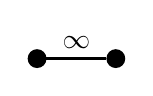
\begin{tikzpicture}
    \begin{scope}[shift={(0,0)}]
        \begin{scope}[every node/.style={circle, fill=black, draw, thick, minimum size = 6pt, inner sep=0pt}]
            \node (1) at (2,-0.5) {};
            \node (2) at (3,-0.5) {};
        \end{scope}

        \begin{scope}[every edge/.style={draw,very thick}]
            \path [-] (1) edge (2);
            \node at (2.5,-0.3) {$\infty$};

        \end{scope}
    \end{scope}
\end{tikzpicture}

This is isomorphic to $\bZ \rtimes S_2$.

For $\bR^2$, for example we can tile the whole space with equilateral triangles. So let it be the chamber and we have a diagram 

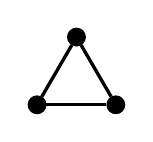
\begin{tikzpicture}
    \begin{scope}[shift={(0,0)}]
        \begin{scope}[every node/.style={circle, fill=black, draw, thick, minimum size = 6pt, inner sep=0pt}]
            \node (1) at (2,-0.5) {};
            \node (2) at (3,-0.5) {};
            \node (3) at (2.5,0.36) {};
        \end{scope}

        \begin{scope}[every edge/.style={draw,very thick}]
            \path [-] (1) edge (2);
            \path [-] (2) edge (3);
            \path [-] (1) edge (3);

        \end{scope}
    \end{scope}
\end{tikzpicture}

This group is isomorphic to $\bZ^2 \rtimes D_6$.

We can tile with hexagon but themselves cannot be chambers, we can split each into 12 30-60-90 triangles. Let them be the chambers and we have a diagram 

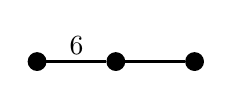
\begin{tikzpicture}
    \begin{scope}[shift={(0,0)}]
        \begin{scope}[every node/.style={circle, fill=black, draw, thick, minimum size = 6pt, inner sep=0pt}]
            \node (1) at (2,-0.5) {};
            \node (2) at (3,-0.5) {};
            \node (3) at (4,-0.5) {};
        \end{scope}

        \begin{scope}[every edge/.style={draw,very thick}]
            \path [-] (1) edge (2);
            \path [-] (2) edge (3);
            \node at (2.5,-0.3) {$6$};

        \end{scope}
    \end{scope}
\end{tikzpicture}

which is the group $\bZ_2 \rtimes D_{12}$.

In fact, for many finite reflection groups $\overline W$ , essential and irreducible, have affine analogous ones. For these groups, let $V$ be the vector space they are acting on of dimension $n$. We can realise $V\rtimes\text{O}(V)$ as an inner semidirect product of $\text{AO}(V)$. Define $L$ to be the $n$-rank lattice of $V$. Then we can define an inner semidirect product $L\rtimes \overline W$ which gives us the affine analogue of $\overline W$. An example is the finite reflection groups of type $A_n$, which can be realised as reflection about planes $x_i-x_j=0$ $(i\neq j)$ in the vector space $V=\{(x_1,\dots,x_n)\in\bR^n:\sum x_i=0\}$ with $\cH := \{x_i-x_j=k:k\in \bZ, i\neq j\}$. One can check $\cH$ in fact gives a Euclidean reflection group with the Coxeter diagram

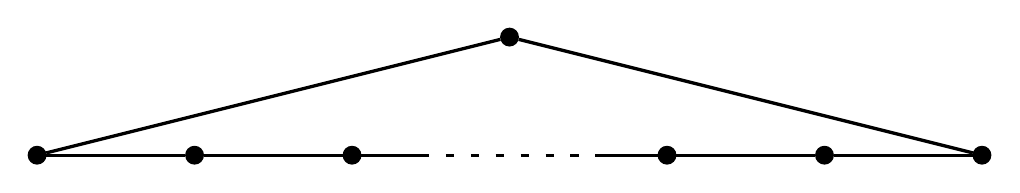
\begin{tikzpicture}
    \begin{scope}[shift={(0,0)}]
        \begin{scope}[every node/.style={circle, fill=black, draw, thick, minimum size = 6pt, inner sep=0pt}]
            \node (1) at (2,0) {};
            \node (2) at (4,0) {};
            \node (3) at (6,0) {};
            \node (n-2) at (10,0) {};
            \node (n-1) at (12,0) {};
            \node (n) at (14,0) {};
            \node (a) at (8,1.5) {};
        \end{scope}
        \node (3a) at (7,0) {};
        \node (3b) at (9,0) {};
        \begin{scope}[every edge/.style={draw,very thick}]
            \path [-] (1) edge (2);
            \path [-] (2) edge (3a);
            \path [loosely dashed] (3a.west) edge (3b.east);
            \path [-] (3b) edge (n-1);
            \path [-] (n-1) edge (n);
            \path [-] (a) edge (1);
            \path [-] (a) edge (n);
        \end{scope}
    \end{scope}
\end{tikzpicture}

with $n$ nodes in the graph.

A non-example is of type $I_2(m)$ except for some specific $m$. There is not way to cover the whole plane using reflections using triangle with an angle $<2\pi/12$ or of $2\pi/7$ for example.

\subsection{Some Model Theory of Euclidean Reflection Groups}


This section follows \cite{MuhlherrPaoliniShelah2022}.

\begin{definition}
    We say a structure $\cN$ is interpretable in $\cM$ if:\begin{enumerate}
        \item The underlying set $A$ is $\{\overline x \in M^k:\cM\models \phi(\overline x)\}$ for some formula $\phi$.
        \item For every function symbols $f(\overline x)$ of $\cN$, there is a formula $\phi$ such that $\cM \models \phi(\overline x,\overline y)$ if and only if $\cN \models f(\overline x)=\overline y$.
    \end{enumerate}
\end{definition}

\begin{definition}
    We say the theory of a group $G$ is decidable if there is an algorithm such that for all sentences $\phi$, it can decide whether $\phi$ is true in $G$.
\end{definition}

For a definition of a sentence and an algorithm, see Appendix \ref{Model Theory}.

\begin{proposition}
\label{thm:interp}
    Euclidean reflection group $G$ is definable in the abelian group $\mathbb Z$ with finitely many parameters.
\end{proposition}

This result follows from the following two lemmas:

\begin{lemma}
    Let $G \cong \mathbb Z^d \rtimes_{\sigma} Q$ where $1\leq d < \omega$, $Q$ is some finite group, and $\theta : Q \rightarrow \text{Aut}(\mathbb Z^d)$ a group homomorphism. $G$ is interpretable in the structure $\mathcal M = (\mathbb Z^d, +, \pi_x)_{x \in Q}$ with finitely many parameters, where $+$ is the normal vector addition and $\pi_x := \sigma(x)$
\end{lemma}

\begin{proof}
    We enumerate $\{\pi_x : x\in Q\}$ as $t_0,\dots,t_{n-1}$ and $t_i := (i,0,\dots,0)$ a $d$-tuple. Let $G=(\mathbb Z^d \times Q,\cdot)$. We represent the universe of $G$ by a tuple $(a,t_i)$ where $a\in M$ and $0\leq i < n$. We need to define the group operation $(a_i,t_i)\cdot(a_j,t_j)=(a_i +_{\mathbb Z^d} t_i(a_j), t_i \cdot_Q t_j)$ in $\mathcal M$. $t_i \cdot_Q t_j$ is definable since $Q$ in finite, we can enumerate all possible product of all elements in $Q$. $a_i +_{\mathbb Z^d} t_i(a_j)$ is definable since $+$ is a built-in function symbol of $\mathcal M$ and $t_i$ is same with $\pi_x$ for some $x$. Again this claim follows from enumerating all possibilities of $t_i$'s.
\end{proof}

\begin{lemma}
    $(\mathbb Z^d, +, \pi_x)_{x \in Q}$ is interpretable in $(\mathbb Z, +, 0)$ with finitely many parameters.
\end{lemma}

\begin{proof}
    Since there are finitely many $\pi_x$'s, it suffices to show we can define $\pi_x$ in $(\mathbb Z, +, 0)$ for some $x\in Q$. $\pi_x$ is an automorphism of $\mathbb Z^d$, which is an $d\times d$ invertible matrix $A$ over $\mathbb Z$.
    $\pi_x(\overline b)=A\overline b$ is a matrix multiplication. We only need to show we can define the element-wise multiplication part is definable. To show this, note that there are only finitely many entries in $A$. The multiplication of $n\times b$ where $n$ is an entry of $A$ and $b$ is an arbitary integer, can be realised as \[
    \underbrace{b+b+\dots+b}_\text{$n$ times}
    \]
    if $n$ is positive and otherwise minus $b$ $-n$ times.
\end{proof}

\begin{theorem}
    Let $W$ be a Euclidean reflection group. Then $Th(W)$ is decidable.
\end{theorem}

\begin{proof}
    $W$ is interpretable in the structure $(\mathbb Z, +, 0)$ with finitely parameters by Proposition \ref{thm:interp}. But all these parameters are integers, so it is interpretable in the structure $(\mathbb Z, +, 0,1)$ with no parameters. We then can translate every sentence in $W$ back to a sentence of $(\mathbb Z, +, 0,1)$. Since the Presburger arithmetic $(\mathbb Z, +, <,0,1)$ is decidable, as a definable structure in its reduct, $Th(W)$ is also decidable.
\end{proof}

\end{document}